%%%%%%%%%%%%%%%%%%%%%%%%%%%%%%%%%%%%%%%%%%%%%%%%%%%%%%%%%%%%%%%%%%%
% v2-CACIC — Estudio empírico de CloudNativePG bajo fallos inyectados
% Formato: Springer LNCS (llncs.cls), A4, ≤10 páginas — CACIC 2026
% Derivado de articulo_angelparejov2-experimental.md (recorte ~49%).
% El marco conceptual (taxonomía, S=(O,K,M,D), invariantes) se externaliza
% al preprint [parejo2026] (v1-6, Zenodo) — cadena de citas anti-salami.
% Compilar: pdflatex main; bibtex no (thebibliography manual); pdflatex x2
%%%%%%%%%%%%%%%%%%%%%%%%%%%%%%%%%%%%%%%%%%%%%%%%%%%%%%%%%%%%%%%%%%%
\documentclass[a4paper]{llncs}

\usepackage[utf8]{inputenc}
\usepackage[T1]{fontenc}
\usepackage{amsmath,amssymb}
\usepackage{graphicx}
\usepackage{booktabs}
\usepackage{array}
\usepackage{url}
\usepackage{hyperref}
\providecommand{\doi}[1]{\url{https://doi.org/#1}}
\renewcommand{\topfraction}{0.9}
\renewcommand{\bottomfraction}{0.9}
\renewcommand{\textfraction}{0.08}
\renewcommand{\floatpagefraction}{0.85}

% Etiqueta de tablas en español (llncs usa "Table" por defecto)
\renewcommand{\tablename}{Tabla}

\begin{document}

\mainmatter

\title{La Visibilidad ante Kubernetes Gobierna el Failover:\\
un Estudio Empírico de CloudNativePG\\ bajo Inyección de Fallos}
\titlerunning{La visibilidad ante Kubernetes gobierna el failover en CloudNativePG}

\author{Angel A. Parejo R.}
\authorrunning{A. A. Parejo R.}
\institute{Universidad de Carabobo, Valencia, Estado Carabobo, Venezuela\\
\email{angelparejo@gmail.com}}

\maketitle

\begin{abstract}
La interacción entre los operadores de PostgreSQL y el almacenamiento
basado en la Container Storage Interface (CSI) en Kubernetes rara vez se
evalúa conjuntamente ante fallos. Sobre un marco descriptivo previo
---taxonomía, vocabulario $S=(O,K,M,D)$ e invariantes de consistencia,
disponibilidad y durabilidad--- este trabajo presenta un estudio empírico de
CloudNativePG mediante inyección de fallos en un clúster productivo,
confrontando lo anticipado con lo observado bajo eliminación del primario (F1),
indisponibilidad sostenida (F2) y partición de red (F3). El hallazgo central:
la variable que gobierna el failover no es el fallo, sino su visibilidad ante
Kubernetes. Eliminar el pod primario dispara la promoción de una réplica (RTO
mediano 7.91~s), pero hacerlo fallar de forma sostenida no promueve ninguna
---el operador recrea el pod en su sitio (36.75~s)---, refutando la expectativa
inicial; la partición preserva la consistencia sin promover. Ninguna transacción
confirmada se perdió (RPO nulo).
\keywords{Kubernetes, PostgreSQL, CloudNativePG, CSI, inyección de fallos,
sistemas distribuidos, consistencia, failover}
\end{abstract}

\section{Introducción}

Kubernetes se ha consolidado como la plataforma de facto para orquestar cargas
en contenedores, incluidas aplicaciones con estado como las bases de datos
\cite{burns2016}. Ello ha impulsado los operadores de
PostgreSQL, que automatizan el ciclo de vida, la replicación y la conmutación
por error (failover) \cite{k8soperator,dobies2020}, y en paralelo la Container
Storage Interface (CSI), que estandariza la integración de backends de
almacenamiento heterogéneos \cite{csi}. La literatura, sin embargo, tiende a
analizar estas capas por separado \cite{bailis2013,gilbert2002,khan2023}, pese
a que la consistencia, la resiliencia y la recuperación ante fallos dependen de
su interacción \cite{avizienis2004}. En un clúster real, la confiabilidad
depende del comportamiento conjunto de la lógica del operador, la planificación
de Kubernetes, la semántica de replicación y las garantías del almacenamiento:
una dependencia multicapa poco explorada, y especialmente relevante bajo fallo.

El argumento de fondo ---que la confiabilidad de las cargas con estado en
Kubernetes es un problema inherentemente multicapa--- y su formalización mediante
una taxonomía, el vocabulario $S=(O,K,M,D)$ y un conjunto de invariantes se
establecen en un trabajo previo de carácter conceptual \cite{parejo2026}. Este
artículo no reintroduce ese marco, sino que lo \emph{confronta con la evidencia}
mediante un estudio empírico de CloudNativePG con inyección controlada de fallos
sobre un clúster productivo, que mide RTO, RPO y visibilidad de transacciones. Sus
contribuciones son: (i)~un hallazgo central ---la variable que gobierna el failover
no es el fallo, sino su \textbf{visibilidad ante Kubernetes}---; en particular, la
indisponibilidad sostenida del primario (\texttt{pod-failure}) \emph{no} promueve
una réplica, en contra de lo anticipado, refutación que es el resultado más
contundente del estudio; y (ii)~la propuesta de extender el marco con un
predicado de visibilidad $V(\text{fallo}, K)$ ---el estado del pod ante el plano de
control: eliminado, \texttt{NotReady}-recreado o \texttt{Ready}--- que el modelo
aún no captura. El alcance está delimitado por las restricciones del clúster
productivo (Sección~\ref{sec:metodologia}).

\section{Trabajos Relacionados}

La literatura relevante se agrupa en tres líneas. La primera, sobre
orquestación, arranca con sistemas como Borg y Omega, que sentaron las bases de
la gestión a gran escala e influyeron en Kubernetes \cite{burns2016};
sobre ellos, CSI estandariza el almacenamiento persistente \cite{csi} y el
patrón \emph{operator} introduce la reconciliación como mecanismo de control
\cite{k8soperator}. La segunda, sobre bases de datos distribuidas, ha tratado
la consistencia y la tolerancia a fallos: CockroachDB evidencia el papel de la
replicación \cite{cockroachdb}, el teorema CAP fija los límites entre
consistencia, disponibilidad y tolerancia a particiones
\cite{bailis2013,gilbert2002}, la taxonomía canónica de la
dependabilidad fija el vocabulario de fallos, errores y fallas
\cite{avizienis2004}. La tercera, sobre recuperación y replicación, destaca el
papel del Write-Ahead Logging (WAL) en la durabilidad
\cite{han2024,stonebraker1991}; más recientemente, el despliegue de
cargas con estado mediante operadores ha ganado atención
\cite{dobies2020,mega2023}, aunque sin caracterizar su comportamiento de
failover, consistencia y durabilidad ante fallos inyectados ---el foco de este
trabajo.

Una cuarta vertiente, metodológica, es la verificación empírica de la
resiliencia mediante inyección controlada de fallos. El \emph{chaos
engineering} propone experimentar deliberadamente con fallos para exponer
debilidades \cite{basiri2016}; la inyección dirigida por linaje automatiza la
búsqueda de combinaciones de fallos que violan garantías \cite{alvaro2018}; y
los estudios sobre particiones de red en producción caracterizan su frecuencia
y severidad \cite{alquraan2018}. Más cerca de este trabajo, el propio proyecto
CloudNativePG incorpora pruebas de caos en su integración continua ---elimina
repetidamente el pod primario para verificar el failover--- pero sin cuantificar
su coste ni distinguir comportamientos \cite{drees2026}; y Chen et al.\ evalúan
la resiliencia del plano de orquestación de Kubernetes inyectando fallos a gran
escala \cite{chen2025}, un objeto distinto del de un operador con estado y su
durabilidad transaccional observable. Existen además comparaciones prácticas
entre operadores publicadas por la industria \cite{portworx},
limitadas a listas de características sin marco formal ni diseño experimental de
inyección de fallos. La brecha no es, pues, la ausencia de inyección de fallos en
Kubernetes, sino la combinación específica de operador de PostgreSQL,
almacenamiento CSI y un verificador de transacciones a nivel de commit que
cuantifica la durabilidad y la consistencia observables.

\section{Marco de Referencia}

El estudio se apoya en un marco descriptivo previo \cite{parejo2026}, del que se
recuerdan aquí solo los elementos necesarios para interpretar los resultados. El
sistema se modela como una tupla $S=(O,K,M,D)$, donde $O$ es la lógica del
operador de PostgreSQL, $K$ el plano de control de Kubernetes, $M$ la capa de
almacenamiento (el «medio» de persistencia) gestionada mediante CSI ---se usa
$M$ y no $C$ para no colisionar con la dimensión de Consistencia del marco--- y
$D$ el motor de base de datos. Más que una formulación cerrada, el modelo captura las interacciones
entre capas y permite razonar sobre cómo una decisión en una capa se propaga al
comportamiento global bajo fallo; el comportamiento emergente se denota
$I(S)=f(O\times K\times M\times D)$ (Fig.~\ref{fig:modelo}). La taxonomía de
operadores (cloud-native como CloudNativePG; basados en Patroni como Zalando;
híbridos como Crunchy), la de almacenamiento CSI (local, distribuido, en red),
las dimensiones de evaluación y la comparación analítica de responsabilidades
de detección y recuperación entre capas por tipo de fallo se desarrollan en
\cite{parejo2026}. El estudio empírico se limita a CloudNativePG por una
restricción del entorno (Sección~\ref{sec:metodologia}) y no mide los demás
operadores.

\begin{figure}[tb]
\centering
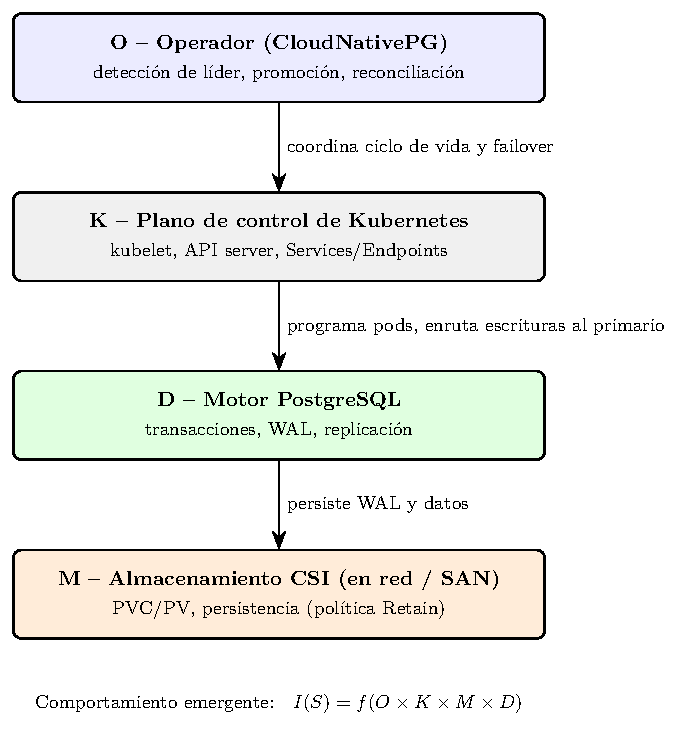
\includegraphics[width=0.55\textwidth]{../figures/fig1_modelo_multicapa}
\caption{Modelo de interacción multicapa $S=(O,K,M,D)$: el operador coordina el
ciclo de vida y el failover a través del plano de control de Kubernetes; el
motor de base de datos persiste el WAL sobre el almacenamiento respaldado por
CSI. Adaptado de \cite{parejo2026}.}
\label{fig:modelo}
\end{figure}

Tres invariantes, definidos en ese marco, caracterizan un comportamiento
aceptable bajo fallo y guían las mediciones de la
Sección~\ref{sec:resultados}: un \emph{invariante de consistencia} ---toda
transacción confirmada debe permanecer accesible tras la recuperación
\cite{bailis2013}---; una \emph{métrica de disponibilidad} ---el RTO se reporta
como cantidad observable por escenario, no como umbral duro, al no haberse
declarado un objetivo de nivel de servicio (SLO) a priori \cite{avizienis2004}---;
y un \emph{invariante de durabilidad} ---toda operación registrada en el WAL debe
ser recuperable tras un fallo \cite{han2024,stonebraker1991}. Cada uno se
operacionaliza mediante métricas observables: RPO, latencia de failover y pérdida
de transacciones.

\section{Metodología Experimental}
\label{sec:metodologia}

\subsection{Entorno, aislamiento y alcance}

Se ejecutó un experimento sobre un clúster Kubernetes en producción (v1.34.6),
con PostgreSQL~16.13 y almacenamiento en red respaldado por el controlador CSI
de Huawei 4.10.1 (\texttt{csi.huawei.com}) sobre Fibre Channel (SAN). La
StorageClass usó política de retención (\texttt{Retain}) y enlace diferido
(\texttt{Wait\-For\-First\-Consumer}); la red se gestionó con Calico~3.31.4. El estudio
se realizó sobre CloudNativePG (CNPG) 1.28.0, exponente del enfoque cloud-native.

El alcance a un único operador responde a una restricción del entorno: el
clúster es productivo y su equipo de operación no permite instalar operadores
nuevos ---como Zalando (Patroni/Spilo) o Crunchy--- por el riesgo sobre las
cargas en producción; el operador CNPG ya presente es, además, compartido con
otros clústeres. El contraste con esos operadores se aborda analíticamente en el
marco de referencia \cite{parejo2026} y se declara trabajo futuro en un entorno no
productivo. La inyección de fallos se realizó con Chaos Mesh~2.8.3, compatible
con la línea 1.34 de Kubernetes; como el entorno está aislado de redes externas
(air-gapped), tanto Chaos Mesh como la imagen del operador se instalaron desde
imágenes importadas localmente.

El experimento corrió en un espacio de nombres dedicado, con cuotas y un alcance
de inyección restringido por control de acceso, de modo que las cargas
productivas quedaron fuera del dominio de fallo. El aislamiento no descansa en la
exclusividad del nodo, sino en tres controles: Chaos Mesh restringido al espacio
de nombres; un doble filtro de selección ---espacio de nombres y nombre de
clúster--- en cada manifiesto de fallo; y una verificación previa (dry-run) que
confirma, por selector, que resuelve exclusivamente a los pods del clúster
experimental. El manifiesto solicita anti-afinidad entre instancias, pero el pool
de nodos elegibles del laboratorio se reducía a un único worker
(\texttt{nodo-lab-01}); en consecuencia, las tres instancias (un primario y dos
réplicas) co-residieron en ese nodo. El failover observado es, por tanto,
intra-nodo, y la tolerancia a un fallo de nodo completo no es testeable por
construcción ---lo que refuerza la lectura del escenario F2 como cota inferior del
RTO ante pérdida de nodo (Secciones~\ref{sec:resultados}
y~\ref{sec:discusion}).

\subsection{Carga de trabajo y cliente de verificación}

El operador desplegó un clúster de tres instancias bajo una carga sintética
continua generada con pgbench (escala \texttt{-s 10}, 4 clientes y 2 hilos), en
rondas de 60~s que toleran failovers. La replicación se mantuvo en su modo
asíncrono por defecto; las cifras de RPO corresponden, pues, a replicación
asíncrona. En paralelo, un cliente de verificación (\texttt{tx-verifier})
registró cada transacción confirmada y comprobó su visibilidad tras la
recuperación: inserta identificadores BIGINT monótonos de un contador propio y
anota cada COMMIT con su marca de tiempo. Ante un fallo reintenta el mismo
identificador en lugar de avanzarlo; así los cortes no introducen huecos
artificiales y un hueco en la tabla de verdad equivale a una escritura reconocida
y perdida, lo que valida la contigüidad de la secuencia como proxy del RPO. La
cadencia es un bucle apretado; ante un fallo aplica una espera de 0.2~s antes de
reintentar, de modo que la granularidad de medición del RTO ---el hueco entre
COMMITs--- es de $\approx$0.2~s. Como el RTO es un hueco medido con el reloj único
del cliente, no depende de la sincronización de relojes entre nodos.

\subsection{Escenarios de fallo y tamaño muestral}

Se aplicaron tres escenarios reproducibles de forma segura en producción:
(i)~\textbf{F1}, eliminación del pod primario, mediante \texttt{PodChaos} en modo
\texttt{pod-kill}; (ii)~\textbf{F2}, indisponibilidad sostenida del primario
durante 10~min, mediante \texttt{PodChaos} en modo \texttt{pod-failure}, como
aproximación observable de un fallo de nodo desde la perspectiva del operador; y
(iii)~\textbf{F3}, partición de red del primario mediante una
\texttt{NetworkPolicy} de Calico ---sin Chaos Mesh---, aplicada y revertida con
\texttt{kubectl}. Se planificó un cuarto escenario (F4): un análisis de
sensibilidad que inyectaría latencia de E/S creciente (0, 20, 50 y 100~ms)
mediante \texttt{IOChaos} a nivel de FUSE; resultó no ejecutable sobre CNPG por
una interacción entre el inyector FUSE y el endurecimiento de seguridad del
operador, y se documenta como lección de instrumentación en la
Sección~\ref{sec:resultados}.

F1 y F2 se repitieron diez veces cada uno ($n=10$). F3 comprendió diez
repeticiones fijas de 60~s, más dos inyecciones exploratorias de mayor duración
(149~s y 300~s) excluidas del cálculo del RTO; la no-promoción se observó en las
doce inyecciones (0/12). El tamaño muestral responde a un compromiso entre las
ventanas de mantenimiento del clúster productivo y la necesidad de estimar
medianas y percentiles; no se realizó un cálculo formal de potencia, y $n=10$ se
declara suficiente para caracterizar tendencia central y dispersión, no para
detectar efectos marginales. Dada la distribución no normal esperada de RTO y
RPO, se reportan medianas y rangos intercuartílicos. Los fallos de nodo genuinos
---desalojo de pods y reasociación (detach/attach) de volúmenes--- no se
reprodujeron: no es posible drenar nodos completos en el clúster productivo, y
las tres instancias co-residían en el único nodo elegible. Por ello el escenario
F2 debe interpretarse como una cota inferior del RTO real ante pérdida de nodo,
no como una réplica completa de dicho evento.

\section{Resultados}
\label{sec:resultados}

Esta sección reporta las mediciones obtenidas al ejecutar la metodología sobre
CloudNativePG. El análisis es esencialmente descriptivo ---medianas, rangos
intercuartílicos e intervalos de confianza de mediana--- y se complementa con una
única prueba de dos grupos, intra-CNPG, que contrasta el RTO de F1 frente al de
F2. La Tabla~\ref{tab:resultados} resume el comportamiento observado.

\subsection{Tiempo de recuperación (RTO) y pérdida de datos (RPO)}

El RPO fue nulo en los tres escenarios, pero su alcance probatorio difiere. Solo
F1 pone a prueba la durabilidad ante un failover real: al promover una réplica,
un RPO nulo implica que ninguna escritura reconocida sobrevivió únicamente en el
primario caído. En F2 y F3 no hubo promoción, de modo que no había divergencia
posible entre primario y réplica y el RPO nulo es trivial. Que CloudNativePG
preserve RPO~=~0 en F1 bajo replicación asíncrona es, por tanto, un hallazgo
genuino ---no una garantía de diseño---, acotado a una carga de escritura modesta:
un \texttt{pod-kill} podría en principio perder WAL confirmado no propagado, pero
bajo esa carga el retardo de replicación era prácticamente nulo en el instante de
la eliminación (inferencia de mecanismo, pues no se registró el LSN lag), de modo
que la réplica promovida ya tenía persistido todo el WAL reconocido
\cite{cnpgdocs}. Además, al residir las tres instancias en el mismo nodo, la
replicación no atravesó un enlace inter-nodo; el RPO~=~0 en F1 no prueba todavía
la durabilidad ante una partición o latencia de red inter-nodo reales
(Sección~\ref{sec:discusion}). Al término del piloto la tabla de verdad resultó
contigua ---identificadores 1 a 613\,253, sin huecos---: ninguna transacción
confirmada se perdió. La variabilidad se concentra, pues, en el tiempo de
recuperación y no en la durabilidad.

\begin{table}[tb]
\centering
\caption{RTO y RPO por escenario de fallo (CloudNativePG). RTO~= tiempo hasta
restablecer la escritura, medido como la mediana del hueco entre transacciones
confirmadas por el cliente de verificación, con granularidad de instrumento
$\approx$0.2~s; RPO~= transacciones confirmadas no visibles tras el fallo. «CP»
denota el comportamiento observado en que el sistema privilegia la consistencia
sobre la disponibilidad (sin split-brain), en sentido operacional y no como
afirmación formal sobre CAP. Tamaños muestrales: F1 y F2, $n=10$; F3, 10
repeticiones fijas más 2 exploratorias excluidas del RTO (no-promoción 0/12).
Fuente: mediciones del piloto.}
\label{tab:resultados}
\begin{tabular}{@{}llll@{}}
\toprule
Escenario & ¿Promueve? & RTO / indisponibilidad & RPO \\
\midrule
F1 --- \texttt{pod-kill} (eliminación) & Sí & 7.91~s (mediana) & 0 \\
F2 --- \texttt{pod-failure} (sostenida) & No & 36.75~s (mediana) & 0 \\
F3 --- partición de red (Calico) & No & $=$ duración de la partición & 0 \\
F4 --- latencia de E/S (IOChaos FUSE) & --- & No ejecutable & --- \\
\bottomrule
\end{tabular}
\end{table}

En la eliminación del primario (F1), CloudNativePG ejecutó un failover en las
diez repeticiones: el nuevo primario aceptó escrituras con un RTO mediano de
7.91~s (rango intercuartílico $\approx[7.62, 8.01]$~s, rango total 6.61--8.17~s;
intervalo de confianza de la mediana $[6.85, 8.15]$~s). La indisponibilidad
sostenida (F2) produjo un comportamiento distinto: en ninguna de las diez
repeticiones hubo promoción. En lugar de promover, el operador recreó el pod
primario en su sitio ---mismo nombre e idéntico PVC--- y lo devolvió a
\texttt{Ready} conservándolo como primario; la ventana de indisponibilidad tuvo
una mediana de 36.75~s (rango intercuartílico $\approx[36.2, 37.1]$~s, rango
total 35.5--38.3~s; IC de la mediana $[36.05, 37.66]$~s). La partición de red
(F3) tampoco disparó promoción: el pod aislado se mantuvo \texttt{Ready} durante
toda la partición y la pérdida de disponibilidad coincidió con su duración
(p.\,ej., 60~s $\to$ 60.75~s de mediana), con recuperación inferior a 1~s al
retirar la \texttt{NetworkPolicy}. Los intervalos de confianza de mediana son de
tipo distribución-libre, con cobertura $\approx$97.9\%.

Por transparencia: la primera inyección de F2 ---corrida de validación previa al
lote--- arrojó una ventana de $\approx$80.5~s y se excluyó de la mediana, de forma
simétrica al tratamiento de las inyecciones exploratorias de F3; la exclusión se
justifica por un efecto de arranque en frío (caché fría, cola de reconciliación no
calentada, primer ciclo de recreación). Dentro del lote de diez se observa una
asociación positiva débil entre el índice de repetición y el RTO (Spearman
$\rho\approx0.62$), que no alcanza significancia con $n=10$ (valor crítico
$\approx0.65$ a $\alpha=0.05$); aun así, la separación entre F1 y F2
($\approx$29~s) es un orden de magnitud mayor que esta variación intra-F2.

De estas mediciones emerge un resultado contraintuitivo: la recuperación tras
eliminar el pod primario (F1) es $\approx$4.6$\times$ más rápida que tras hacerlo
fallar de forma sostenida (F2), pese a tratarse del mismo componente (razón de
medianas 4.65$\times$: 36.75~s frente a 7.91~s). La separación entre ambas
distribuciones es completa: una prueba de Mann--Whitney entre F1 y F2 ($n=10$ por
grupo) arroja $U=0$, con un valor $p$ exacto bilateral $\approx1.1\times10^{-5}$,
correlación rango-biserial 1.00 y sin solapamiento; la diferencia de medianas,
estimada mediante Hodges--Lehmann, es de 28.96~s. El mecanismo es que el
\texttt{pod-kill} elimina el pod y dispara una promoción inmediata, mientras el
\texttt{pod-failure} induce al operador a esperar y recrear el pod en su sitio
antes de restablecer el servicio. La no-promoción en F2 (0/10) y F3 (0/12) admite
una cota superior por intervalo binomial exacto (Clopper--Pearson): con 95\% de
confianza, la probabilidad real de promoción es $\le$25.9\% para 0/10 y
$\le$22.1\% para 0/12; no obstante, la conclusión se apoya sobre todo en el
mecanismo observado y no únicamente en el conteo.

El hallazgo central que articula los tres comportamientos es que la variable que
determina el failover en CloudNativePG no es el fallo en sí, sino su
\textbf{visibilidad ante Kubernetes}. En F1, la muerte del contenedor deja el pod
en \texttt{NotReady}; el operador registra el evento «Current primary isn't
healthy, initiating a failover» y promueve en $\approx$7.9~s. En F3, las sondas
del kubelet no se bloquean ---el failsafe de Calico preserva el tráfico de
host---, el pod aislado permanece \texttt{Ready}, el operador no emite evento y no
promueve: elige consistencia sobre disponibilidad (comportamiento CP) sin
split-brain. F2 refina el mecanismo: aunque el pod queda \texttt{NotReady}, se
recrea con la misma identidad y PVC, y el operador prefiere esperar esa
recreación antes que promover. La promoción de F1 se explica, por tanto, por la
\textbf{eliminación} del pod ---el primario deja de existir--- y no por el mero
estado \texttt{NotReady}.

\subsection{Sensibilidad a la latencia de E/S: una lección de instrumentación}

El escenario F4 resultó no ejecutable sobre CloudNativePG, y ese bloqueo es en sí
un resultado. El inyector FUSE \texttt{toda} de Chaos Mesh realiza un
\texttt{ptrace attach} sobre el proceso de PostgreSQL, pero al montar el sistema
de archivos FUSE falla con \texttt{Read-only file system (os error 30)} y entra
en un ciclo de reintentos. La causa es que CloudNativePG endurece sus pods con
\texttt{readOnly\-Root\-Filesystem: true} ---junto con \texttt{runAsNonRoot} y el
descarte de capacidades---, mientras \texttt{toda} requiere un sistema de
archivos raíz escribible. La configuración era correcta (el dry-run resolvió
exclusivamente a los pods del clúster experimental); no se trata de un error de
configuración, sino de una incompatibilidad entre el inyector FUSE de Chaos Mesh
y el \texttt{readOnly\-Root\-Filesystem} de CloudNativePG. Se registra estrictamente
como una limitación de instrumentación observada con este par concreto de
herramientas, no como una propiedad general. La medición cuantitativa de la
sensibilidad a la E/S queda como trabajo futuro; dos vías la harían viable: un
test confirmatorio que desactive \texttt{readOnly\-Root\-Filesystem}, y la limitación
de ancho de banda de E/S a nivel de cgroup (\texttt{io.max}), que no depende de
FUSE ni modifica el sistema bajo prueba.

\subsection{Contraste entre el comportamiento anticipado y el observado}

El marco de referencia \cite{parejo2026} anticipaba, a partir del comportamiento
documentado, que el fallo del pod primario dispara la promoción de una réplica:
F1 lo confirma ---casi trivialmente---, pero el aporte de mayor peso es la
refutación en F2, ya expuesta. Los tres escenarios comparten una variable de
control que el marco no captura de forma explícita: la visibilidad del fallo ante
Kubernetes. De ahí que se proponga extender $S=(O,K,M,D)$ con un predicado
$V(\text{fallo}, K)$ que registre el estado del pod primario ---eliminado (F1),
\texttt{NotReady}-recreado (F2) o \texttt{Ready} (F3)--- como la dimensión que
ordena el gradiente de RTO observado. El bloqueo de F4 apunta a una segunda
extensión: la observabilidad e inyectabilidad de los fallos dependen del
endurecimiento del operador, interacción que el modelo tampoco recoge. No se
reclama una validación del marco, sino una caracterización empírica que lo
confronta con el comportamiento observado y señala hacia dónde extenderlo.

\section{Discusión}
\label{sec:discusion}

La confiabilidad en entornos cloud-native es un fenómeno inherentemente
multicapa: decisiones aparentemente locales ---la selección de un operador o de
un tipo de almacenamiento--- tienen implicaciones globales en RTO, RPO o la
visibilidad de las transacciones, un impacto que la literatura en sistemas
distribuidos rara vez atribuye a la orquestación y a abstracciones de
almacenamiento como CSI \cite{gilbert2002,bailis2013,avizienis2004}.

El trabajo presenta limitaciones que delimitan el alcance de sus resultados. El
estudio empírico cubre un único operador (CloudNativePG) y una única categoría de
almacenamiento ---CSI en red, SAN sobre Fibre Channel--- con hardware homogéneo,
por la restricción del entorno productivo; la comparación entre operadores y
categorías se aborda analíticamente en el marco de referencia \cite{parejo2026}.
De forma crítica, el fallo de nodo no se reproduce como tal: las tres instancias
co-residían en el único nodo elegible, por lo que el failover observado es
intra-nodo. Esa co-localización acota además el RPO nulo de F1 ---la replicación
no atravesó un enlace inter-nodo, así que no prueba todavía la durabilidad ante
latencia de red inter-nodo real---, y F2 no captura la latencia de reasociación
(detach/attach) del volumen CSI, dominante en un fallo de nodo genuino; por ello
sus cifras son una cota inferior del RTO real. Por último, F4 no fue ejecutable
por la interacción entre el endurecimiento del operador y el inyector FUSE.

\section{Conclusiones}
\label{sec:conclusiones}

Este trabajo confrontó empíricamente un marco descriptivo multicapa
\cite{parejo2026} con el comportamiento observado de CloudNativePG mediante
inyección controlada de fallos sobre un clúster productivo. El hallazgo central es
que la variable que gobierna el failover no es el fallo en sí, sino su visibilidad
ante Kubernetes: la refutación de que la indisponibilidad sostenida del primario
promovería una réplica ---no lo hizo en ninguna de las diez repeticiones--- es su
resultado de mayor fuerza probatoria, y motiva extender el marco con un predicado
de visibilidad $V(\text{fallo}, K)$. Ninguna transacción confirmada se perdió (RPO
nulo), si bien solo F1 pone a prueba la durabilidad ante un failover real. El
aporte entrega una lectura operacional ---la visibilidad como variable de control
del failover--- reutilizable para evaluar configuraciones distintas de la aquí
medida. Como trabajo futuro se plantea incorporar otros operadores (Zalando/Patroni
y Crunchy) en un entorno no productivo, contrastar las categorías de almacenamiento
local y distribuido, reproducir un fallo de nodo genuino y medir la sensibilidad
del RTO a la latencia de E/S mediante un mecanismo que no dependa de FUSE.

\subsubsection*{Disponibilidad de datos y código.}
Los datos limpios de RTO/RPO por escenario y el paquete de ejecución ---manifiestos
del clúster y de Chaos Mesh, el cliente verificador de transacciones, la carga
pgbench y los scripts de análisis, junto con los registros crudos--- se facilitan
a petición. El experimento se ejecutó sobre un clúster productivo bajo acceso
restringido, por lo que el entorno no es de acceso público; el material permite
reproducir el diseño en un clúster equivalente.

\begin{thebibliography}{99}
\setlength{\itemsep}{0pt}

\bibitem{burns2016}
Burns, B., Grant, B., Oppenheimer, D., Brewer, E., Wilkes, J.: Borg, Omega, and
Kubernetes. ACM Queue \textbf{14}(1), 70--93 (2016)

\bibitem{csi}
Kubernetes: Container Storage Interface (CSI) (2024),
\url{https://kubernetes.io}

\bibitem{cockroachdb}
Taft, A., et al.: CockroachDB: The resilient geo-distributed SQL database. In:
Proc. ACM SIGMOD, pp. 1493--1509 (2020)

\bibitem{k8soperator}
Kubernetes: Operator pattern. Kubernetes Documentation,
\url{https://kubernetes.io/docs/concepts/extend-kubernetes/operator/}. Consultado
el 8 de julio de 2026

\bibitem{bailis2013}
Bailis, P., Ghodsi, A.: Eventual consistency today: limitations, extensions, and
beyond. Communications of the ACM \textbf{56}(5), 55--63 (2013)

\bibitem{gilbert2002}
Gilbert, S., Lynch, N.: Brewer's conjecture and the feasibility of consistent,
available, partition-tolerant web services. ACM SIGACT News \textbf{33}(2),
51--59 (2002)

\bibitem{avizienis2004}
Avizienis, A., Laprie, J.-C., Randell, B., Landwehr, C.: Basic concepts and
taxonomy of dependable and secure computing. IEEE Trans. Dependable and Secure
Computing \textbf{1}(1), 11--33 (2004)

\bibitem{khan2023}
Khan, W., Kumar, T., Zhang, C., Raj, K., Roy, A.M., Luo, B.: SQL and NoSQL
database software architecture performance analysis and assessments---a
systematic literature review. Big Data and Cognitive Computing \textbf{7}(2),
art. 97 (2023). \doi{10.3390/bdcc7020097}

\bibitem{han2024}
Han, F., et al.: PALF: Replicated write-ahead logging for distributed databases.
Proc. VLDB Endowment \textbf{17}(12), 3745--3758 (2024).
\doi{10.14778/3685800.3685803}

\bibitem{stonebraker1991}
Stonebraker, M., Kemnitz, G.: The POSTGRES next-generation database management
system. Communications of the ACM \textbf{34}(10), 78--92 (1991)

\bibitem{dobies2020}
Dobies, J., Wood, J.: Kubernetes Operators: Automating the Container
Orchestration Platform. O'Reilly Media, Sebastopol (2020)

\bibitem{mega2023}
Mega, C.: Orchestrating information governance workloads as stateful services
using Kubernetes operator framework. In: Service-Oriented Computing (SummerSOC
2023). CCIS, vol. 1847, pp. 125--143. Springer, Cham (2023).
\doi{10.1007/978-3-031-45728-9_8}

\bibitem{basiri2016}
Basiri, A., Behnam, N., de Rooij, R., Hochstein, L., Kosewski, L., Reynolds, J.,
Rosenthal, C.: Chaos engineering. IEEE Software \textbf{33}(3), 35--41 (2016)

\bibitem{alvaro2018}
Alvaro, P., Tymon, S.: Abstracting the geniuses away from failure testing.
Communications of the ACM \textbf{61}(1), 54--61 (2018)

\bibitem{alquraan2018}
Alquraan, A., Takruri, H., Alfatafta, M., Al-Kiswany, S.: An analysis of
network-partitioning failures in cloud systems. In: Proc. 13th USENIX OSDI, pp.
51--68 (2018)

\bibitem{cnpgdocs}
CloudNativePG: CloudNativePG Documentation (2026),
\url{https://cloudnative-pg.io/docs/}. Consultado el 7 de julio de 2026

\bibitem{portworx}
Portworx: Choosing a Kubernetes operator for PostgreSQL,
\url{https://portworx.com/blog/choosing-a-kubernetes-operator-for-postgresql/}

\bibitem{drees2026}
Drees, F.: Chaos testing the CloudNativePG project. CloudNativePG Blog, 5 de
enero de 2026, \url{https://cloudnative-pg.io/blog/lfx-chaos-testing-yash-agarwal/}.
Consultado el 8 de julio de 2026

\bibitem{chen2025}
Chen, Z., Goudarzi, M., Toosi, A.N.: Resilience evaluation of Kubernetes in
cloud-edge environments via failure injection. arXiv:2507.16109 [cs.DC] (2025)

\bibitem{parejo2026}
Parejo R., A.A.: Hacia un análisis multicapa de operadores de PostgreSQL y
almacenamiento CSI en Kubernetes: taxonomía, modelo formal y protocolo
experimental reproducible. Preprint, Zenodo (2026).
\url{https://doi.org/10.5281/zenodo.XXXXXXX}

\end{thebibliography}

\end{document}
